\section{Bayes' theorem}

Bayes' theorem describes the probability of an event to occur, depending on the prior knowledge of conditions related to the event \citep{bayesBasic}. 
\begin{equation}
\label{eqn:bayesianTheorem}
P(A|B) = \frac{P(B|A)P(A)}{P(B)}.
\end{equation}
P(A|B) is the posterior probability of A given that B is true. P(B|A) is called conditional probability of B given A being true. P(A) is the prior probability, the probability of A occurring without any additional information. Finally P(B) is the marginal probability of B without any given condition. This theorem is often used for Bayesian inference where it expresses how a belief, which is represented as probability changes due to related evidence.	

\section{Bayesian inference}
\label{section:bayesianInference}

Bayesian inference is a process of data analysis to calculate the probability of a hypothesis depending on the available related evidence. As over time more and more evidence becomes available the probabilities can be updated yielding a more sophisticated view on the hypothesis. It is given, according to Bayes' theorem, by
\begin{equation}
\label{eqn:bayesianInference}
P(H|E) = \frac{P(E|H)P(H)}{P(E)},
\end{equation}
where H represents a hypothesis and E some related evidence. P(H|E) is the posterior probability which signifies the probability of the hypothesis after the evidence was observed. P(E|H) is called likelihood and it is the probability of observing the evidence 	given the hypothesis. It is a measure of the compatibility of the observed evidence with the given hypothesis. P(H) is the prior probability which is the probability of the hypothesis before any evidence is considered or obtained. P(E) is called marginal likelihood that represents the probability of the evidence being observed. However it is the same independent of the chosen hypothesis. Thus, it is not factored in when comparing different hypotheses.
Bayesian inference could be applied to the "face in shadow" example of Section \ref{section:feedbackInVisualCortex}. There a neuron sees a small part of the visual field and signals if it sees an edge or not. At first it has the evidence of the observed pixels available and from it can calculate the likelihood that an edge is present. Together with the prior knowledge of how probable an edge being present is, it can conclude the posterior probability for the hypothesis "there is an edge". Later when the related evidence that there is a face in the picture is being fed back from the inferior temporal cortex this additional information updates the posterior probability. The additional evidence $E_2$ that is being fed back can be added to the calculation by
\begin{equation}
\label{eqn:bayesianInference}
P(H|E_2) = \frac{P(E_2|E)P(E|H)P(H)}{P(E_2)}.
\end{equation}
\citep{bayesInferenceBook}

\section{Network model}

The network model used for the experiments in this thesis was taken from \citet{nessler} and expanded by an additional layer to include some hierarchical feedback information.

\paragraph{Neuron model}
As in \citet{nessler} the input neurons X are firing according to a poisson process with an average firing rate $f_{input}$ when active and with 0 Hz when in an inactive state. The input neurons receive a binary input, for example a black or white pixel of an image. The excitatory post synaptic potentials (EPSPs) $x_i(t)$ that these neurons produce can be seen in Figure \ref{fig:XSpike}. A double exponential kernel was used to generate the EPSP. The kernel has a time constant for the rise of the signal $\tau_{rise}$  and a time constant for the decay of the signal $\tau_{decay}$. The addition of the time step size $\delta t$ was necessary to get the time t at the end of the current simulation step. $t_f$ is the time at which the spike of $x_i$ occurred
\begin{equation}
\label{eqn:EPSP}
x_i(t) = e^{-(t + \delta t - t_f) / \tau_{decay}} - e^{-(t + \delta t - t_f) / \tau_{rise}}.
\end{equation}

\begin{figure}
  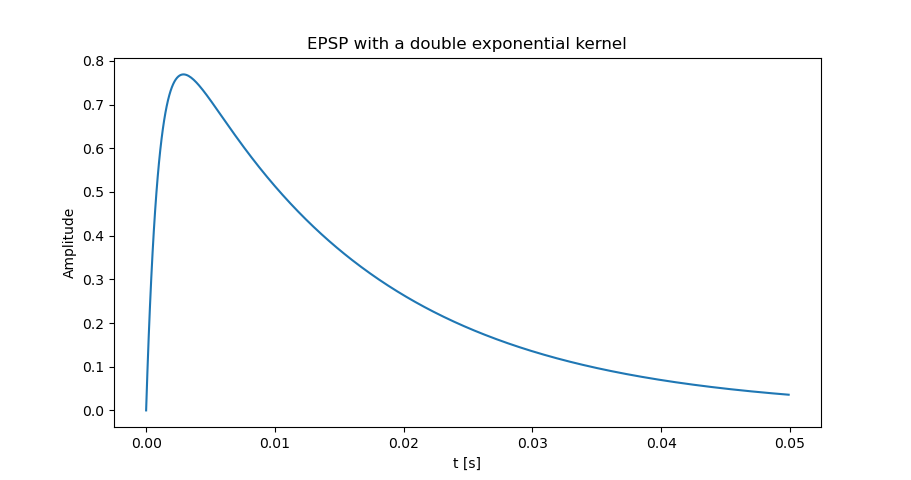
\includegraphics[width=\linewidth]{figures/XSpike.png}
  \caption{Form of an excitatory post synaptic potential generated by an input neuron over time. A double exponential kernel was used to generate this signal. These signals are fed to the next layer of the network. }
  \label{fig:XSpike}
\end{figure}

The firing rate of an output neuron $y_k$ is given by
\begin{equation}
\label{eqn:rk}
r_k(t) = e^{u_k(t) - I(t)}.
\end{equation}
The probability of an individual output neuron to fire within a time step $\delta t$ is given by
\begin{equation}
\label{eqn:rkdt}
r_k(t) \cdot \delta t.
\end{equation}

\paragraph{Network architecture}
Each pixel of an input image was connected to two neurons. The first of these neurons is in an active state when the pixel is black and in an inactive state otherwise. The second neuron expresses the opposite behaviour. As a consequence the network needs ($width \cdot height \cdot 2$) excitatory input neurons $x_1,...,x_n$. These input neurons are fully connected to the excitatory output neurons $y_1,...,y_k$. This means that that every input neuron $x_i$ is connected to each output neuron $y_k$. The membrane potential $u_k$ of each output neuron is calculated by multiplying the EPSP of each input neuron times the weight of the connection between them
\begin{equation}
\label{eqn:uk}
u_k(t) = \sum_{i=1}^n w_{ki} \cdot x_i(t).
\end{equation}
In \citet{nessler} each output neuron $y_k$ also had an intrinsic excitability $w_{k0}$ which was learned for each neuron. For the experiments of this thesis however it was omitted, as the different classes of  input images were equally likely, thus the intrinsic excitability of each output neuron would end up being the same.
The output neurons are modelled in a winner-takes-all (WTA) circuit. The WTA behaviour was implemented via an adaptive inhibition signal. The adaptive inhibition is used to regulate
the membrane potentials of the output neurons so that all of them together fire with a total firing rate $R(t) = 200 Hz$ on average. Due to that there never is a time window in which no output neuron may fire. However, it is unlikely for an output neuron to fire right after another output neuron has fired.

\paragraph{Inhibition}
The inhibition signal was chosen to depend on the current membrane potential of the output neurons. According to \citet{nessler} the total firing rate of the output neurons is
\begin{equation}
\label{eqn:R}
R(t) = \sum_{k=1}^K e^{u_k(t) - I(t)}.
\end{equation}
Solving this equation for I(t) yields
\begin{equation}
\label{}
R(t) = \frac{ \sum_{k=1}^K e^{u_k(t)}}{e^{I(t)}}
\end{equation}
\begin{equation}
\label{}
e^{I(t)} = \frac{\sum_{k=1}^K e^{u_k(t)}}{R(t)}
\end{equation}
\begin{equation}
\label{}
I(t) = \ln{ \frac{ \sum_{k=1}^K e^{u_k(t)}}{R(t)}}
\end{equation}
\begin{equation}
\label{eqn:I(t)}
I(t) =  - \ln{R(t)} + \ln{  \sum_{k=1}^K e^{u_k(t)}}.
\end{equation}

At every timestep of the simulation in Equation in Equation \ref{eqn:rk} the inhibition signal I(t) is subtracted from the membrane potential $u_k(t)$ of every output neuron. Due to that the membrane potentials are altered to always yield a spiking frequency of 200 Hz, regardless if it would be too low or too high without it. This means that the adaptive inhibition signal can also function as an excitatory signal. 

\paragraph{Spike timing dependent plasticity}
The weights $w_{ki}$ between neurons $x_i$ and $y_k$ are updated whenever an output neuron fires. The time window $\sigma$, after which spikes are no longer considered, was set to 10 ms according to \citet{nessler}. If $y_k$ produces a spike all its weights are updated as
\begin{equation}
\label{deltawki}
\Delta w_{ki} = \begin{dcases*} \lambda \cdot (ce^{-w_{ki}} - 1) & if $x_{i}$ fired in $ [t^f - \sigma, t^f] $ \\
\lambda \cdot (-1) & \text{if $ x_i $ did not fire in $ [t^f - \sigma, t^f] $, } \end{dcases*}
\end{equation}
where $\lambda$ is the learning rate, the parameter c shifts the weight values, $t^f$ is the time when $y_k$ spiked and $\sigma$ is the time window in which input spikes are considered as "before" an output spike. As the membrane potentials $u_k$ of the output neurons result from the addition of the EPSPs of the input neurons times the corresponding weight, a way to control the average size of u is needed. If u is too small the output neurons will fire too sparsely and if u is too big it will impair the learning process. So to limit u, the size of the weights is controlled via the parameter c. The learning rate $\lambda$ is needed to control the size of each weight update. If it is too big few output neurons will respond to multiple input classes and others will only respond too little or not at all. On the other hand if $\lambda$ is too small the network will learn very slowly and may never converge. 

\section{Connection between synaptic weights and Bayes inference}

1. Nessler : If the STDP-induced changes in
synaptic strength depend in a particular way on the current
synaptic strength, STDP approximates for each synapse exponentially fast the conditional probability that the presynaptic neuron
has fired just before the postsynaptic neuron (given that the
postsynaptic neuron fires). This principle suggests that synaptic
weights can be understood as conditional probabilities, and the
ensemble of all weights of a neuron as a generative model for high-dimensional inputs that - after learning - causes it to fire with a
probability that depends on how well its current input agrees with
this generative model. The concept of a generative model is well
known in theoretical neuroscience [26,27]
 In a Bayesian inference context, every input
spike provides evidence for an observed variable, whereas every
output spike represents one stochastic sample from the posterior
distribution over hidden causes encoded in the circuit.

2.Nessler showed that STDP is able to approximate expectation maximization, by creating implicit generative models in the synaptic weights.

3. this is unsupervised learning, output neurons autonomously specialize on a hidden cause (due to learning rule)

Mathe:

!!!! equation (4.15) (after The additional prior layer resulted in an) is missing a sum of l !!!!!




